\section{停留时间分布}


\begin{frame}
    \frametitle{停留时间分布}

    化学反应进行的完全程度与反应物料在反应器内停留时间的长短有关，时间越长，反应进行得越完全，可见，研究反应物料在反应器内的停留时间问题具有十分重要的意义。

    通常所说的停留时间是指流体以进入系统时算起，到其离开系统时为止，在系统内总共经历的时间，即流体从系统的进口至出口所耗费的时间。
    \begin{itemize}
        \item 间歇反应器不存在停留时间分布问题
        \item 连续操作反应器，不同粒子停留时间是否相同？
        \begin{itemize}
            \item[\bullet] 活塞流反应器 \qquad $\surd$ 
            \item[\bullet] 连续釜式反应器 \quad $\times$ 
        \end{itemize}
    \end{itemize}

\end{frame}


\begin{frame}
    \frametitle{两种停留时间分布}

    \begin{itemize}
        \item 寿命分布
        
        流体粒子从进入系统起到离开系统止，在系统内停留的时间。
        \item 年龄分布
        
        对留存在系统中的流体粒子而言，从进入系统算起在系统中停留的时间。
    \end{itemize}
    \begin{figure}
        \centering
        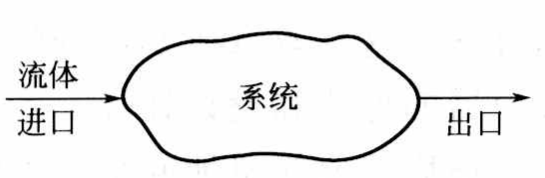
\includegraphics[width=.8\linewidth]{figures/fig5.1.png}
    \end{figure}
   

\end{frame}


\begin{frame}
    \frametitle{停留时间分布的定量描述}

    \begin{minipage}{0.48\linewidth}
        \begin{figure}
            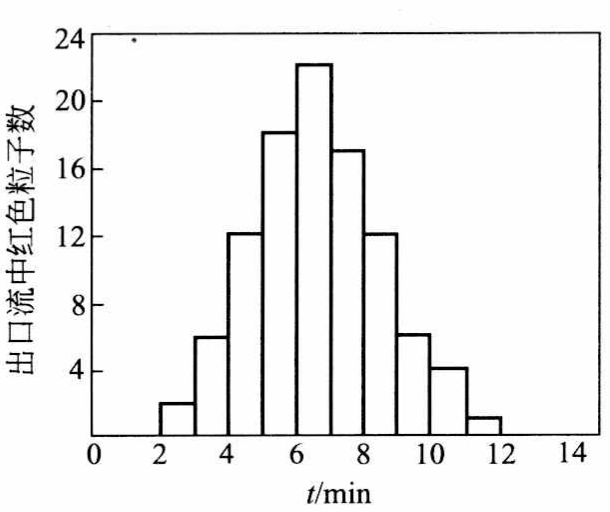
\includegraphics[width=\linewidth]{figures/fig5.2.png}
            \caption{停留时间分布直方图}
        \end{figure}
    \end{minipage}\hfill
    \begin{minipage}{0.48\linewidth}
        \begin{enumerate}
            \item 某时刻向入口加入100个红色粒子
            \item 在出口处记录不同时间间隔内流出的红色粒子数
            \item 根据观察结果作图
        \end{enumerate}
    \end{minipage}

\end{frame}


\begin{frame}
    \frametitle{停留时间分布的定量描述}
    \begin{minipage}{0.48\linewidth}
        \begin{figure}
            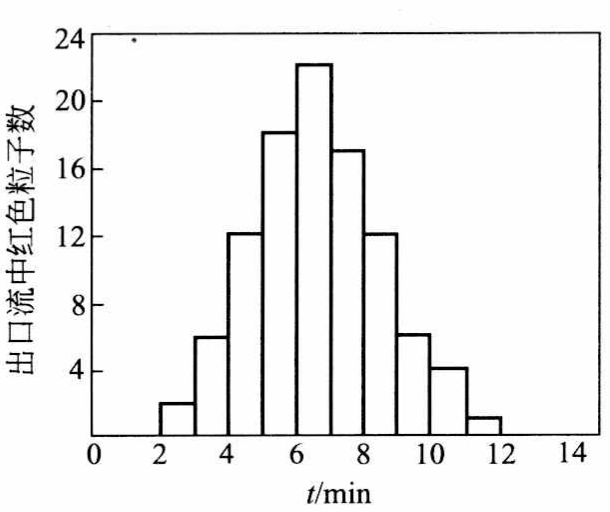
\includegraphics[width=\linewidth]{figures/fig5.2.png}
            \caption{停留时间分布直方图}
        \end{figure}
    \end{minipage}\hfill
    \begin{minipage}{0.48\linewidth}
        红色粒子由恒定流量$Q$的流体带入系统。
        
        $N_i$ 表示第 i 个时间段$\Delta t_i$流出系统的单位流体体积中红色粒子的个数。
        
        粒子的总个数 $N_\mathrm{t}=100$。
        
        各时间间隔内红色粒子所占分率之和为
        \[
            \sum_{i=0}^{\infty}\frac{QN_{i}}{N_{t}}\Delta t_{i}=\frac{1}{N_{t}}\sum_{i=0}^{\infty}QN_{i}\Delta t_{i}
        \]
        当$\Delta t_i \to 0$时，
        \[
            \frac{QN_{i}}{N_{t}} = E(t) \quad \mathrm{s^{-1}}
        \]
    \end{minipage}
\end{frame}


\begin{frame}
    \frametitle{停留时间分布密度函数}

    \begin{minipage}{0.44\linewidth}
        \begin{figure}
            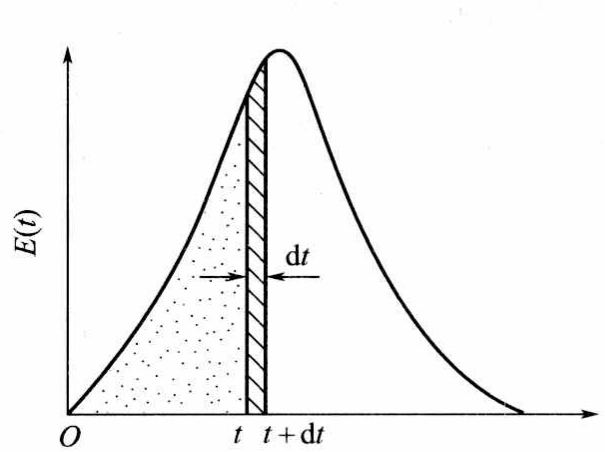
\includegraphics[width=\linewidth]{figures/fig5.3.png}
            \caption{停留时间分布密度函数}
        \end{figure}
    \end{minipage}\hfill
    \begin{minipage}{0.52\linewidth}
        \begin{enumerate}
            \item 改用红色流体作示踪剂
            \item 连续检测出口流中红色流体的浓度
            \item 观察结果将是一条连续的停留时间分布曲线
        \end{enumerate}
    \end{minipage}

    $E(t) \dif t$表示流体粒子在系统内的停留时间介于$t$到$t+\dif t$之间的概率。

    $E(t)$叫做停留时间分布密度函数，其量纲是[时间]$^{-1}$。

\end{frame}


\begin{frame}
    \frametitle{停留时间分布函数}

    \begin{minipage}{0.44\linewidth}
        \begin{figure}
            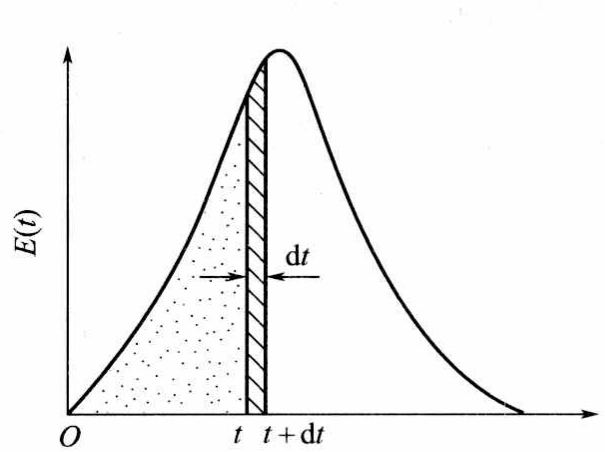
\includegraphics[width=\linewidth]{figures/fig5.3.png}
            \caption{停留时间分布密度函数}
        \end{figure}
        
    \end{minipage}\hfill
    \begin{minipage}{0.52\linewidth}
        \[
        E(t)=0 \qquad (t<0)
    \]
    \[
        E(t)\geqslant 0 \qquad (t\geqslant 0)
    \]
    \[
        \int_0^\infty E(t)\dif t =1
    \]
    \[
        \int_0^t E(t)\dif t = F(t)
    \]
    \end{minipage}

    $F(t)$叫做停留时间分布函数，其意义是停留时间小于$t$的流体粒子所占的分数。

    从概率论的角度，$F(t)$表示流体粒子的停留时间小于$t$的概率。

\end{frame}


\begin{frame}
    \frametitle{停留时间分布的定量描述}

    \begin{minipage}{0.46\linewidth}
        \begin{figure}
            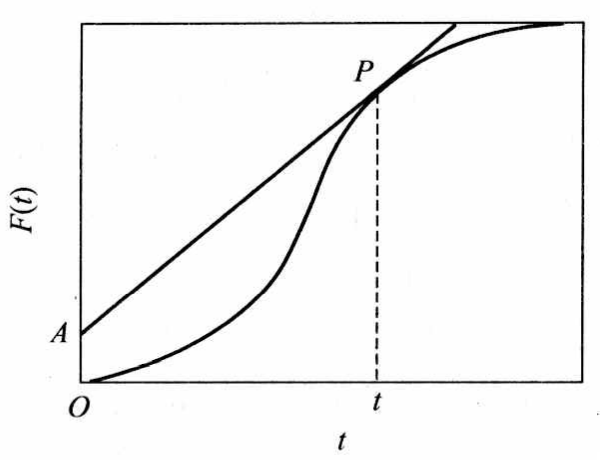
\includegraphics[width=\linewidth]{figures/fig5.4.png}
            \caption{停留时间分布函数}
        \end{figure}        
    \end{minipage}\hfill
    \begin{minipage}{0.48\linewidth}
        \begin{itemize}
            \item $F(t)$曲线是一条单调递增的线
            \item $F(t)$最大值为1，$F(\infty) =1$
            \item $F(t) =0 \qquad (t \leqslant 0)$
        \end{itemize}

        \[
            E(t) = \frac{\dif F(t)}{\dif t}
        \]
    \end{minipage}

    

\end{frame}


\begin{frame}
    \frametitle{$E(t)$和$F(t)$的关系}
    \begin{figure}[htpb]
        \centering
        \setcounter{subfigure}{0}
        \subfloat[$F(t) = \int_0^t E(t)\dif t$]{
\includegraphics[height=4.5cm]{fig5.3.png}}\quad
        \subfloat[$E(t) = \frac{\dif F(t)}{\dif t}$]{
\includegraphics[height=4.5cm]{fig5.4.png}}
    \end{figure}
    \begin{itemize}
      \item 若$E(t)$曲线已知，将其进行积分即得相应的$F(t)$值。
      \item 若$F(t)$曲线已知，在线上的一点作切线，该直线的斜率即等于相应的$E(t)$值。
    \end{itemize}
\end{frame}


\begin{frame}
    \frametitle{无因次停留时间}

    有时为了应用上方便，常常使用无因次停留时间$\theta$
    \[
        \theta = \frac{\ t\ }{\bar{t}}
    \]
    式中$\bar{t}$为平均停留时间，对于在闭式系统中流动的流体，当流体密度维持不变时，其平均停留时间等于
    \[
        \bar{t} = \frac{V_\mathrm{r}}{Q}
    \]
    如果一个流体粒子的停留时间介于区间$(t$，$t+\dif t)$内，则它的无因次停留时间也一定介于区间$(\theta$，$\theta+\dif \theta)$内，因为这所指的是同一事件。
    \[
        E(t)\dif t = E(\theta)\dif \theta 
    \]

\end{frame}


\begin{frame}
    \frametitle{停留时间分布无因次化}

    $E(\theta)$与$E(t)$的关系为
    \[
        E(\theta) = \bar{t} E(t)
    \]
    $F(t)$本身是一累积概率，
    \[
        F(\theta) = F(t)
    \]
    \[
        \begin{aligned}
            &\int_0^\infty E(\theta)\dif \theta =1   \\
            &\int_0^\theta E(\theta)\dif \theta = F(\theta) \\
            &E(\theta) = \frac{\dif F(\theta)}{\dif \theta}
        \end{aligned}
    \]

\end{frame}